\documentclass[UTF8,fontset=none,zihao=-4,openany]{ctexrep}

\usepackage[a4paper,top=21mm,bottom=22mm,left=20mm,right=20mm,headheight=15pt]{geometry}
\usepackage{fontspec}
\IfFontExistsTF{Songti SC}{
  \setCJKmainfont{Songti SC}
}{
  \setCJKmainfont{FandolSong-Regular}
}
\IfFontExistsTF{PingFang SC}{
  \setCJKsansfont{PingFang SC}
}{
  \setCJKsansfont{FandolHei-Regular}
}
\IfFontExistsTF{STKaiti}{
  \setCJKmonofont{STKaiti}
}{
  \setCJKmonofont{FandolKai-Regular}
}
\IfFontExistsTF{Avenir Next}{
  \setmainfont{Avenir Next}
  \setsansfont{Avenir Next}
}{
  \setmainfont{TeX Gyre Heros}
  \setsansfont{TeX Gyre Heros}
}
\setmonofont{Menlo}[Scale=0.88]

\usepackage{xcolor}
\usepackage{graphicx}
\usepackage{booktabs}
\usepackage{tabularx}
\usepackage{longtable}
\usepackage{array}
\usepackage{colortbl}
\usepackage{enumitem}
\usepackage{fancyhdr}
\usepackage{environ}
\usepackage{listings}
\usepackage{pdflscape}
\usepackage{tikz}
\usetikzlibrary{mindmap,positioning,arrows.meta,fit,backgrounds,shapes.geometric}
\usepackage{hyperref}

\definecolor{OCNavy}{HTML}{14213D}
\definecolor{OCBlue}{HTML}{2563EB}
\definecolor{OCTeal}{HTML}{0F766E}
\definecolor{OCGreen}{HTML}{2F855A}
\definecolor{OCOrange}{HTML}{D97706}
\definecolor{OCRed}{HTML}{C2413A}
\definecolor{OCPurple}{HTML}{7C3AED}
\definecolor{OCInk}{HTML}{1F2937}
\definecolor{OCMuted}{HTML}{667085}
\definecolor{OCLight}{HTML}{F4F7FB}
\definecolor{OCLine}{HTML}{D7DEE8}
\definecolor{OCGold}{HTML}{F0B429}

\hypersetup{
  colorlinks=true,
  linkcolor=OCBlue,
  urlcolor=OCTeal,
  citecolor=OCPurple,
  pdftitle={OpenChronicle x Vida: clean-room function parity report},
  pdfauthor={OpenChronicle Vida Integration},
  pdfsubject={Engineering status, ecosystem research, architecture, evaluation and roadmap},
  pdfkeywords={OpenChronicle, Vida, local-first, desktop agent, Action Plane, Workspace Cleanup}
}

\pagestyle{fancy}
\fancyhf{}
\fancyhead[L]{\sffamily\small OpenChronicle $\times$ Vida Clean-room 复现报告}
\fancyhead[R]{\sffamily\small 2026-08-23 / \texttt{bf34152}}
\fancyfoot[C]{\sffamily\small\thepage}
\renewcommand{\headrulewidth}{0.35pt}
\renewcommand{\footrulewidth}{0pt}

\setlist[itemize]{leftmargin=2em,itemsep=0.28em,topsep=0.4em}
\setlist[enumerate]{leftmargin=2.2em,itemsep=0.32em,topsep=0.4em}
\renewcommand{\arraystretch}{1.24}
\setlength{\tabcolsep}{5pt}
\setlength{\parindent}{2em}
\setlength{\parskip}{0.15em}
\sloppy

\newcolumntype{Y}{>{\raggedright\arraybackslash}X}
\newcolumntype{C}[1]{>{\centering\arraybackslash}p{#1}}
\newcolumntype{R}[1]{>{\raggedleft\arraybackslash}p{#1}}
\newcommand{\code}[1]{\texttt{\detokenize{#1}}}
\newcommand{\good}{\textcolor{OCGreen}{\bfseries 已验证}}
\newcommand{\inprogress}{\textcolor{OCOrange}{\bfseries 进行中}}
\newcommand{\openitem}{\textcolor{OCRed}{\bfseries 未完成}}

\newcommand{\boxedcontent}[3]{%
  \begin{center}%
  \setlength{\fboxsep}{4mm}%
  \fcolorbox{#1}{#2}{%
    \begin{minipage}{0.91\linewidth}%
    #3%
    \end{minipage}%
  }%
  \end{center}%
}
\NewEnviron{executivebox}{\boxedcontent{OCBlue}{OCLight}{\BODY}}
\NewEnviron{riskbox}{\boxedcontent{OCRed!65}{OCRed!4}{\BODY}}
\NewEnviron{decisionbox}{\boxedcontent{OCGreen!75}{OCGreen!5}{\BODY}}

\lstset{
  basicstyle=\ttfamily\small,
  backgroundcolor=\color{OCLight},
  frame=single,
  rulecolor=\color{OCLine},
  breaklines=true,
  columns=fullflexible,
  keepspaces=true,
  showstringspaces=false,
  xleftmargin=1em,
  xrightmargin=1em,
  aboveskip=0.8em,
  belowskip=0.8em
}

\begin{document}

\begin{titlepage}
\begin{tikzpicture}[remember picture,overlay]
  \fill[OCNavy] (current page.north west) rectangle ([yshift=-8.8cm]current page.north east);
  \fill[OCBlue] ([yshift=-8.8cm]current page.north west) rectangle ([yshift=-9.05cm]current page.north east);
  \draw[OCBlue!16,line width=0.7pt] ([xshift=15mm,yshift=-22mm]current page.north west)
    grid[xstep=13mm,ystep=13mm] ([xshift=-15mm,yshift=-84mm]current page.north east);
  \fill[OCTeal!18] ([xshift=-34mm,yshift=-28mm]current page.north east) circle (28mm);
  \fill[OCBlue!18] ([xshift=-18mm,yshift=-67mm]current page.north east) circle (17mm);
\end{tikzpicture}

\vspace*{18mm}
{\sffamily\bfseries\color{white}\fontsize{29}{36}\selectfont
OpenChronicle $\times$ Vida\par}
\vspace{3mm}
{\sffamily\bfseries\color{white}\fontsize{22}{29}\selectfont
基于公开证据的 Clean-room 功能复现完整报告\par}
\vspace{8mm}
{\sffamily\color{white!85}\Large
工程现状、竞品与开源生态、信任架构、验收合同及后续路线\par}

\vfill
\begin{executivebox}
\begin{tabularx}{\textwidth}{>{\bfseries\sffamily\color{OCNavy}}p{35mm}Y}
报告快照 & 2026-08-23（Asia/Shanghai）\\
代码基线 & \code{agent/vida-integration} @ \code{bf3415223456a869c5020d50c7766c79f0df3f1c}\\
上游基线 & \code{Einsia/OpenChronicle} @ \code{bad3a1e86d8e85a82d76d3883a491abc06f8c6b7}\\
协作入口 & Draft PR \href{https://github.com/chimeraHHH/OpenChronicle/pull/10}{chimeraHHH/OpenChronicle\#10}\\
研究边界 & Vida 官方公开页面、公开法律文本、公开仓库与当前分支；不使用私有接口、二进制逆向或非公开材料\\
\end{tabularx}
\end{executivebox}

\vspace{11mm}
{\sffamily\large\color{OCMuted}
OpenChronicle Vida Integration Engineering Report\par}
\vspace{2mm}
{\sffamily\color{OCMuted}
LaTeX / XeLaTeX / TikZ mind map / reproducible PDF\par}
\end{titlepage}

\pagenumbering{roman}
\chapter*{执行摘要}
\addcontentsline{toc}{chapter}{执行摘要}

\begin{executivebox}
\textbf{结论先行。} 截至报告快照，OpenChronicle 已从上游的本地屏幕上下文记忆工具，演进为一个具有隐私防火墙、可审查记忆、来源证明、主动建议内核和多项 Prepare 工作流的本地优先桌面助手原型。Vida 公开列出的五个核心用例中，Daily Wrap、Prompt Rescue、Reply Rescue 和 Resume Rescue 已有可运行、可审查、无自动外部提交能力的工程切片；Workspace Cleanup 仍未实现。因此，本项目\textbf{尚不能宣称已经完成 Vida 公开功能复现}，下一关键路径是可逆 Action Plane 及其第一个受控文件整理用例。
\end{executivebox}

本轮工作形成了四项可复核结论：

\begin{enumerate}
  \item \textbf{产品方向没有偏移。} 复现目标是 Vida 公开可观察的工作流和主动循环，而不是复制其品牌、视觉资产、代码或推测私有实现。OpenChronicle 保留本地优先 Memory Plane，并新增独立 Action Plane。
  \item \textbf{当前实现具有真实纵深。} 相对上游基线，当前分支包含 71 个提交、386 个变更文件；新增量中包含依赖锁、Tauri ACL schema 和生成物，不能把 129,036 行新增简单等同于手写业务代码。
  \item \textbf{当前回归是绿色的。} 在 macOS 当前环境中，Python 测试 1,185 项、React/TypeScript 测试 50 项、Rust/Tauri 测试 48 项全部通过。开发包记录过 11 步 Resume Rescue 端到端检查和精确 PDF 页面预览，但仍是 ad-hoc 签名，尚未完成 Developer ID、公证和正式发布门禁。
  \item \textbf{下一步不是让 LLM 直接整理文件。} 竞品与源码审计表明，预览、规则分类和撤销已有成熟参考，但路径批准通常没有绑定内容身份和执行时状态。OpenChronicle 应先实现确定性的只读清单和计划，再实现摘要绑定、短时批准、即时重检、原子同卷移动、结果证明和严格撤销；LLM 分类只能在安全执行内核之后接入。
\end{enumerate}

\vspace{2mm}
\noindent\textbf{当前成熟度一览}

\begin{center}
\begin{tabularx}{\textwidth}{p{37mm}C{24mm}Y}
\toprule
能力 & 状态 & 证据边界 \\
\midrule
可信观察、隐私与运行时 & \inprogress & 大量失效关闭与故障测试已落地；独立红队仍发现进程后代、挂起时钟等需复核问题 \\
可审查记忆与 Daily Wrap & \good & 来源链、候选审查、遗忘、时间线和本地日总结已覆盖 CLI/MCP/桌面读取 \\
Suggestion Kernel / Work Resumption & \good & 无副作用建议、去重/预算/证据绑定的工程切片已存在；不等同于长期真实用户质量验证 \\
Prompt Rescue & \good & 选择/粘贴输入、无工具生成、编辑/复制、硬删除；不自动提交 \\
Reply Rescue & \good & 会话目标绑定、审查和复制；不自动发送 \\
Resume Rescue & \good & 资料审查、JSON Resume 互操作、PDF/DOCX 提取、监督改写、确定性 PDF、精确页面预览与原生保存 \\
Workspace Cleanup / Action Plane & \openitem & 仅有研究与验收合同；尚无用户工作区文件执行能力 \\
正式分发 & \openitem & 开发包可审计；签名、公证、受控更新和 Windows 端未完成 \\
\bottomrule
\end{tabularx}
\end{center}

\tableofcontents
\clearpage
\pagenumbering{arabic}

\chapter{任务定义与研究方法}

\section{复现目标}

Vida 的公开站点把产品定义为能够理解上下文、预判意图并交付成果的主动代理，并公开列出 Reply Rescue、Prompt Rescue、Resume Rescue、Workspace Cleanup 和 Daily Wrap 五个用例\cite{vida-home}。本项目采用下面的可验证定义：

\begin{decisionbox}
“复现 Vida”不是像素级克隆，也不是宣称性能超过不可测的闭源产品；它表示 OpenChronicle 在自己的本地优先信任模型下，完成上述五个公开工作流，并让每个工作流通过预先冻结的隐私、来源、批准、副作用、结果验证和恢复门禁。
\end{decisionbox}

本报告把 OpenChronicle 自有的 Work Resumption 保留为第六个附加工作流。它重建中断前的工作状态；Vida 的 Resume Rescue 则明确指求职简历准备\cite{vida-home}，两者不能混名。

\section{证据等级}

为避免把宣传、代码和实测混成一个结论，报告使用四级证据：

\begin{enumerate}
  \item \textbf{P1 官方公开证据：} Vida 官网、隐私政策、服务条款；仅用于确定公开功能面和厂商声明。
  \item \textbf{P2 上游源码证据：} 固定到 commit 的公开仓库、许可证和实际实现；用于比较机制，不复制受限制代码。
  \item \textbf{P3 当前分支证据：} OpenChronicle 源码、内部设计文档、版本化夹具与 commit 历史。
  \item \textbf{P4 本机实测证据：} 2026-08-23 在当前 macOS 环境运行的 Python、TypeScript 和 Rust 回归，以及此前冻结在提交中的开发包审计记录。
\end{enumerate}

Vida 的 “SOTA Achieved”、客户评价和 “production-grade” 均属于 P1 厂商声明，不是独立基准结果。公开隐私政策说明：在用户授权后，产品可能处理应用名、窗口标题、可见文本、选择内容、控件和工作流信号，并可能把相关内容传给第三方模型提供商\cite{vida-privacy}。OpenChronicle 因而不复制 Vida 的数据流，而以本地 canonical data、最小化 egress 和来源可追踪性作为差异化约束。

\section{版本固定与可复现性}

报告绑定当前分支 \code{bf34152}。生态仓库使用 2026-08-23 GitHub 默认分支 HEAD 快照；附录~\ref{app:repos} 列出精确 SHA。所有结论均是时间点结论，后续使用前应重新拉取并对比变更。

\chapter{Vida 公开产品面与 Clean-room 验收解释}

\section{公开可观察能力}

\begin{longtable}{p{31mm}p{54mm}p{74mm}}
\toprule
公开能力 & Vida 官方描述 & OpenChronicle 的可测试解释 \\
\midrule
\endfirsthead
\toprule
公开能力 & Vida 官方描述 & OpenChronicle 的可测试解释 \\
\midrule
\endhead
Reply Rescue & 理解会话上下文，生成可立即使用的回复 & 冻结一个精确会话/收件人快照，生成可编辑草稿；源变化即失效；首个 pilot 永不发送 \\
Prompt Rescue & 在 AI 看到前升级粗糙问题 & 绑定当前选择和项目证据，分离用户文本/检索证据/生成方案；可复制但不自动提交 \\
Resume Rescue & 把经历、文档和上下文转成面向真实机会的简历 & 用户显式选择资料与职位快照；每个可见事实绑定审查过的证据；无依据时显示缺口，绝不申请投递 \\
Workspace Cleanup & 把混乱文件和桌面变成清晰、可预览结构 & 只扫描用户批准根目录；展示精确移动/重命名 diff、冲突、文件数和字节；批准后才执行，并支持结果证明和撤销 \\
Daily Wrap & 自动把一天转成清晰的进展和成果总结 & 使用本地日期/时区和来源窗口生成可追踪版本；迟到数据产生修订而非覆盖历史 \\
主动循环 & 学习上下文、跨应用拼接、提出动作、按边界 Suggest/Prepare/Act & 机会检测、证据检索、去重/冷却/打扰预算、准备产物、确定性策略、可信批准、能力代理、验证和审计 \\
记忆控制 & 可查看、编辑、删除 About Me 记忆 & 记忆条目必须可读、可追源、可编辑/替代/永久遗忘；删除要使依赖建议和产物失效 \\
\bottomrule
\end{longtable}

\section{首个 pilot 的自治边界}

\begin{center}
\begin{tabularx}{\textwidth}{p{36mm}p{32mm}Y}
\toprule
工作流 & 初始自治级别 & 明确禁止 \\
\midrule
Daily Wrap & Suggest & 不以总结内容发消息或创建外部任务 \\
Prompt / Reply / Resume Rescue & Prepare & 不提交提示、不发送消息、不投递申请 \\
Work Resumption & Suggest / Prepare & 不自动打开、修改或运行外部项目 \\
Workspace Cleanup & Prepare, then approved Act & 不永久删除、不跨卷移动、不跟随逃逸 symlink、不执行任意 shell \\
\bottomrule
\end{tabularx}
\end{center}

发送、发布、支付、凭据使用、永久删除和不受限 shell 均不属于五用例 pilot。把这些能力提前加入会扩大权限面，却不会提高公开工作流验收可信度。

\chapter{总体架构与思维导图}

\section{Memory Plane 与 Action Plane 分离}

OpenChronicle 保持 Memory Plane 为事实和证据来源；Action Plane 负责副作用。屏幕或文档中的文本永远是\textbf{不可信数据}，不能成为 capability、policy 或 approval。

\begin{figure}[htbp]
\centering
\begin{tikzpicture}[
  node distance=8mm and 8mm,
  box/.style={rounded corners=2mm, draw=OCLine, line width=0.8pt, fill=white, minimum height=10mm, text width=28mm, align=center, font=\sffamily\small},
  memory/.style={box, draw=OCTeal, fill=OCTeal!5},
  prepare/.style={box, draw=OCBlue, fill=OCBlue!5},
  action/.style={box, draw=OCOrange, fill=OCOrange!6},
  trust/.style={box, draw=OCGreen, fill=OCGreen!6},
  future/.style={box, draw=OCOrange, fill=OCOrange!3, dashed},
  arrow/.style={-{Stealth[length=2.2mm]}, line width=0.8pt, draw=OCMuted}
]
\node[memory] (watch) {AX watcher\\快捷键/计时器};
\node[trust, right=of watch] (privacy) {隐私防火墙\\窗口身份绑定};
\node[memory, right=of privacy] (obs) {版本化\\Observation};
\node[memory, below=of obs] (timeline) {Timeline / Session\\Memory / Provenance};
\node[prepare, left=of timeline] (context) {ContextService\\证据活性检查};
\node[prepare, left=of context] (planner) {Suggestion Kernel\\Typed Planner};
\node[future, below=of planner] (policy) {确定性策略\\风险分类};
\node[future, right=of policy] (approval) {可信批准 UI\\短时 token};
\node[future, right=of approval] (broker) {隔离能力代理\\move / rename};
\node[future, right=of broker] (verify) {postcondition\\audit / undo};
\draw[arrow] (watch) -- (privacy);
\draw[arrow] (privacy) -- (obs);
\draw[arrow] (obs) -- (timeline);
\draw[arrow] (timeline) -- (context);
\draw[arrow] (context) -- (planner);
\draw[arrow] (planner) -- (policy);
\draw[arrow] (policy) -- (approval);
\draw[arrow] (approval) -- (broker);
\draw[arrow] (broker) -- (verify);
\node[fit=(watch)(privacy)(obs)(timeline)(context)(planner), draw=OCTeal!45, rounded corners=3mm, inner sep=4mm, label={[font=\sffamily\bfseries\color{OCTeal}]above:已实现的本地 Memory / Prepare 平面}] {};
\node[fit=(policy)(approval)(broker)(verify), draw=OCOrange!55, dashed, rounded corners=3mm, inner sep=4mm, label={[font=\sffamily\bfseries\color{OCOrange}]below:下一阶段 Action Plane}] {};
\end{tikzpicture}
\caption{Clean-room 主动助手架构。虚线区域是 Workspace Cleanup 的必要前置，不是当前已完成能力。}
\end{figure}

\section{TikZ 思维导图}

下面的思维导图把产品目标、已实现平面、下一行动平面、证据交付和生态参照放在同一张图上。图源独立保存在 \code{reports/figures/vida-mindmap.tikz}，可单独编译。

\begin{landscape}
\thispagestyle{empty}
\begin{center}
\vspace*{4mm}
{\sffamily\bfseries\LARGE\color{OCNavy} OpenChronicle $\times$ Vida 功能复现思维导图}\par
\vspace{3mm}
\resizebox{!}{0.78\textheight}{\begin{tikzpicture}[
  x=1cm,
  y=1cm,
  root/.style={
    circle,
    draw=OCNavy!85,
    line width=1.2pt,
    fill=OCNavy,
    text=white,
    minimum size=4.4cm,
    text width=3.8cm,
    align=center,
    font=\sffamily\bfseries\fontsize{14}{18}\selectfont
  },
  topic/.style={
    circle,
    draw=white,
    line width=1.1pt,
    text=white,
    minimum size=3.0cm,
    text width=2.45cm,
    align=center,
    font=\sffamily\bfseries\normalsize
  },
  leaf/.style={
    rounded corners=3mm,
    draw=white,
    line width=0.9pt,
    text=white,
    minimum width=3.4cm,
    minimum height=1.15cm,
    text width=2.9cm,
    align=center,
    font=\sffamily\bfseries\scriptsize,
    inner sep=2.3mm
  },
  branch/.style={line width=7pt, line cap=round},
  twig/.style={line width=3pt, line cap=round},
]

\node[root] (root) at (0,0) {OpenChronicle\\Vida 公开功能\\Clean-room\\复现};

\node[topic,fill=OCBlue] (product) at (-7,-3) {产品目标};
\node[leaf,fill=OCBlue] (product-a) at (-10.7,-4.6) {五个公开核心用例};
\node[leaf,fill=OCBlue] (product-b) at (-10.7,-3.0) {主动理解上下文};
\node[leaf,fill=OCBlue] (product-c) at (-10.7,-1.4) {可控记忆与操作};

\node[topic,fill=OCTeal] (memory) at (0,-5.1) {Memory Plane\\记忆平面};
\node[leaf,fill=OCTeal] (memory-a) at (-3.4,-7.45) {AX 观察\\隐私防火墙};
\node[leaf,fill=OCTeal] (memory-b) at (0,-7.45) {时间线\\会话归约};
\node[leaf,fill=OCTeal] (memory-c) at (3.4,-7.45) {来源证明\\可审查记忆};

\node[topic,fill=OCGreen] (prepare) at (7,-3) {Prepare / Suggest\\准备型工作流};
\node[leaf,fill=OCGreen] (prepare-a) at (10.7,-4.6) {Daily Wrap\\Work Resumption};
\node[leaf,fill=OCGreen] (prepare-b) at (10.7,-3.0) {Prompt Rescue\\Reply Rescue};
\node[leaf,fill=OCGreen] (prepare-c) at (10.7,-1.4) {Resume Rescue\\精确预览导出};

\node[topic,fill=OCOrange] (action) at (7,3) {Action Plane\\行动平面};
\node[leaf,fill=OCOrange] (action-a) at (10.7,1.4) {类型化计划\\确定性策略};
\node[leaf,fill=OCOrange] (action-b) at (10.7,3.0) {精确批准\\即时重检};
\node[leaf,fill=OCOrange] (action-c) at (10.7,4.6) {执行证明\\审计与撤销};

\node[topic,fill=OCRed] (evidence) at (0,5.1) {证据与交付};
\node[leaf,fill=OCRed] (evidence-a) at (-3.4,7.45) {版本化夹具\\故障矩阵};
\node[leaf,fill=OCRed] (evidence-b) at (0,7.45) {Python / TS / Rust\\全栈回归};
\node[leaf,fill=OCRed] (evidence-c) at (3.4,7.45) {打包审计\\签名公证};

\node[topic,fill=OCPurple] (ecosystem) at (-7,3) {生态参考};
\node[leaf,fill=OCPurple] (ecosystem-a) at (-10.7,1.4) {Vida 官方公开证据};
\node[leaf,fill=OCPurple] (ecosystem-b) at (-10.7,3.0) {本地记忆\\桌面 Agent};
\node[leaf,fill=OCPurple] (ecosystem-c) at (-10.7,4.6) {文件整理\\治理与基准};

\begin{scope}[on background layer]
  \draw[branch,OCBlue!72] (root) -- (product);
  \draw[twig,OCBlue!72] (product) -- (product-a);
  \draw[twig,OCBlue!72] (product) -- (product-b);
  \draw[twig,OCBlue!72] (product) -- (product-c);

  \draw[branch,OCTeal!72] (root) -- (memory);
  \draw[twig,OCTeal!72] (memory) -- (memory-a);
  \draw[twig,OCTeal!72] (memory) -- (memory-b);
  \draw[twig,OCTeal!72] (memory) -- (memory-c);

  \draw[branch,OCGreen!72] (root) -- (prepare);
  \draw[twig,OCGreen!72] (prepare) -- (prepare-a);
  \draw[twig,OCGreen!72] (prepare) -- (prepare-b);
  \draw[twig,OCGreen!72] (prepare) -- (prepare-c);

  \draw[branch,OCOrange!72] (root) -- (action);
  \draw[twig,OCOrange!72] (action) -- (action-a);
  \draw[twig,OCOrange!72] (action) -- (action-b);
  \draw[twig,OCOrange!72] (action) -- (action-c);

  \draw[branch,OCRed!72] (root) -- (evidence);
  \draw[twig,OCRed!72] (evidence) -- (evidence-a);
  \draw[twig,OCRed!72] (evidence) -- (evidence-b);
  \draw[twig,OCRed!72] (evidence) -- (evidence-c);

  \draw[branch,OCPurple!72] (root) -- (ecosystem);
  \draw[twig,OCPurple!72] (ecosystem) -- (ecosystem-a);
  \draw[twig,OCPurple!72] (ecosystem) -- (ecosystem-b);
  \draw[twig,OCPurple!72] (ecosystem) -- (ecosystem-c);
\end{scope}
\end{tikzpicture}
}
\end{center}
\end{landscape}

\section{信任边界}

\small
\noindent\begin{tabularx}{\textwidth}{>{\raggedright\arraybackslash}p{34mm}>{\raggedright\arraybackslash}p{51mm}Y}
\toprule
边界 & 允许 & 禁止 \\
\midrule
观察边界 & 获得权限后读取受策略允许的窗口身份、AX 文本和可选截图 & 屏幕回退、身份不一致的截图、被排除应用数据落盘 \\
模型 egress & 仅发送当前工作流选择并经政策审查的最小数据 & 整段历史、未审查记忆、凭据、文件系统能力、任意工具 \\
WebView & 显示闭合 schema 的派生产物和精确 PNG 页面 & 原始本地路径、任意文件读写、把不可信 HTML 注入 DOM \\
Native shell & 显式命令、严格请求 schema、Tauri ACL、原生选择/保存对话框 & 通用 shell、通用路径写权限、由 WebView 自报执行成功 \\
Action broker（未来） & 计划摘要绑定的同根目录 move/rename，验证后写收据 & 永久删除、跨卷复制、symlink 逃逸、批准后改参数 \\
\bottomrule
\end{tabularx}
\normalsize

\chapter{当前工程成果}

\section{Stage 0：可信观察、隐私和运行时}

当前分支把原始桌面观察改造成显式的信任管线：

\begin{itemize}
  \item watcher debounce 保存深拷贝快照，并把持久化触发投影成精确窗口身份；
  \item capture 文件名、时间戳和 observation ID 可往返，私有文件原子写入；
  \item 策略先于 AX 读取，浏览器 URL 规则使用稳定标识并失效关闭；
  \item 截图默认关闭；开启时绑定 app、bundle、title、PID、\code{CGWindowID} 和 bounds，不允许 display fallback；
  \item classifier 交付使用 SQLite outbox 和 receipt，崩溃/重试不把失败伪装成成功；
  \item daemon、provider worker、超时/终止和代际切换具备故障注入测试；
  \item macOS AX helper、selection helper、Tauri sidecar 和打包清单均进入版本控制。
\end{itemize}

这是一组强工程基础，但不是完成声明。第~\ref{sec:risks} 节列出的独立审计问题说明，发布前仍需复核成功 worker 残留后代、suspend 边界时钟取样和历史扫描复杂度。

\section{Stage 1：可审查记忆、来源和 Daily Wrap}

实现包括：

\begin{itemize}
  \item SQLite 时间线与 session canonical state，Markdown 作为可读长期记忆；
  \item evidence reference、policy digest、source revision 和 provenance graph；
  \item memory candidate 的 approve / reject / edit / forget 状态机，以及永久遗忘失效传播；
  \item ContextService 对 active、retired、tampered 和 policy-mismatched 证据进行活性校验；
  \item 以本地日期和时区为边界的 Daily Wrap，迟到证据创建 revision；
  \item CLI、只读 MCP 和 Tauri 桌面端的来源抽屉、隐私控制、时间线和审查页。
\end{itemize}

关键产品属性不是“模型能总结”，而是用户能回答：这条记忆来自哪里、当时政策是什么、源是否仍有效、删除后哪些产物会失效。

\section{Stage 2：Suggestion Kernel 与 Work Resumption}

Suggestion Kernel 已具备类型化建议、证据引用、去重、冷却、每日打扰预算和 durable transitions。Work Resumption 从会话与时间线中提出“最后验证状态、未完成项、下一步”，不把推断伪装成观察事实。当前 suggestion 接受按钮只记录 acknowledgement，不执行外部动作。

版本化基准位于 \code{benchmarks/vida-suggestions-v1}，包含 reactive control、deterministic heuristic control 和完整内核对比。其目标是先守住精度、来源覆盖和无副作用，再讨论 recall。

\section{Prompt Rescue}

Prompt Rescue 的工程边界是“准备，不提交”：

\begin{itemize}
  \item 支持手动粘贴和 macOS 聚焦选择，选择内容带应用/窗口身份；
  \item 输入、检索上下文和生成提案分区显示，屏幕文本标记为不可信；
  \item provider worker 不获得工具，只接收政策允许的最小 envelope；
  \item 结果使用闭合 schema、digest 和 current-state 检查，可编辑、重试、复制和硬删除；
  \item 前端和后端都拒绝非 \code{none} 的 \code{action_capability}。
\end{itemize}

\section{Reply Rescue}

Reply Rescue 复用 Prepare 平面，但把输入绑定到一个明确 thread / recipient snapshot。quoted text 仍是 untrusted evidence；目标或源内容变化会使草稿失效。初始版本可审查、编辑和复制，任何 send 路径均不存在。

\section{Resume Rescue}

Resume Rescue 是当前最完整的垂直切片，其数据流为：

\begin{center}
\code{reviewed facts + opportunity snapshot -> preflight -> supervised rewrite -> claim verification -> deterministic render -> exact preview -> native save}
\end{center}

\subsection{资料与事实模型}

\begin{itemize}
  \item 用户显式选择简历资料和职位说明；资料默认不自动进入 master profile；
  \item PDF 与 DOCX 提取保留页码/边界框或 OOXML part/block provenance；
  \item JSON Resume import 以字段路径、未知字段、遗漏原因和 loss ledger 呈现，所有候选初始未选择；
  \item admission 重新解析原始输入，并同时检查 review digest 与 target profile CAS；
  \item master fact、opportunity snapshot、projection、rewrite proposal 和 export 各自版本化。
\end{itemize}

\subsection{监督改写与事实约束}

云端或本地模型只获得用户选择的职位和已审查事实。模型没有文件、浏览器或提交工具。每条 proposal 单独接受/拒绝；unsupported claim 或 missing evidence 不进入最终简历。评分只报告需求覆盖与事实支持，不宣称 ATS 通过率、求职成功率或招聘偏好。

\subsection{确定性 PDF 与精确预览}

当前实现固定 ReportLab、HarfBuzz、PDFium 和字体资产，服务端先生成并审计 PDF，再由 PDFium 栅格化为最多 20 页、单页最多 4 MiB、总计最多 20 MiB、最大边长 2048 的 PNG。响应绑定 projection digest、artifact digest、semantic preview digest 和 PDF content digest。Rust 端再次验证闭合 schema、页序、尺寸、base64、PNG 签名/IEND、逐页 SHA-256 与总量限制。

原生保存要求调用者提供\textbf{刚刚预览过的精确 PDF content digest}；Rust 重新生成并确认摘要完全一致，才打开 save dialog。WebView 不接触 PDF 原始字节和本地源路径，也不向 DOM 注入简历 HTML。协议版本为 v15。

\subsection{桌面与开发包}

React/Tauri/Python sidecar 形成三层边界：WebView 只处理闭合派生数据；Rust 负责原生命令和 ACL；Python 负责领域逻辑、来源校验和渲染。构建清单与 Tauri permission 文件有一致性测试，防止命令在 release tree-shaking 中被移除。开发包的冻结端到端流程记录 11 个操作通过，并完成深层 ad-hoc code-sign 验证；由于没有 Developer ID 和 notarization，release gate 正确保持为 false。

\chapter{竞品与开源仓库调研}

\section{调研分层}

广泛参考不等于把所有项目放进依赖。仓库被分成四类：

\begin{enumerate}
  \item \textbf{观察与记忆：} ActivityWatch、screenpipe、Windrecorder；
  \item \textbf{本地桌面 Agent：} Coworker、OpenAdapt Flow；
  \item \textbf{文件整理与文件系统：} AI File Sorter、FolderSorter、organize、Spacedrive；
  \item \textbf{评估：} LongMemEval-V2、OSWorld-V2。
\end{enumerate}

\section{机制比较}

\small
\begin{longtable}{p{26mm}p{40mm}p{51mm}p{36mm}}
\toprule
项目 & 值得参考的机制 & 源码审计边界 & 采用方式 \\
\midrule
\endfirsthead
\toprule
项目 & 值得参考的机制 & 源码审计边界 & 采用方式 \\
\midrule
\endhead
ActivityWatch & 本地活动采集、事件桶、查询与成熟生态 & 不是跨应用语义记忆或行动代理 & 行为/负载参考，不替换 AX 语义管线 \\
screenpipe & 本地连续屏幕/音频、搜索和插件生态 & 更大的截图与媒体隐私面 & 作为连续记忆竞品，拒绝默认全屏捕获 \\
Windrecorder & 长周期本地录屏、OCR、检索 & 主要是回放/检索，不是来源约束行动 & 作为留存与存储压力参考 \\
Coworker & 用户选择文件夹、原生 approval card、每次写操作暂停、任务日志 & permission request 主要包含 operation/path/target/500 字符 preview 和 5 分钟超时；未见内容摘要、目标负证明、批准 digest 或 postcondition & 采用文件夹授权与易懂审批 UX；独立设计精确批准 \\
OpenAdapt Flow & authorization / identity / postcondition / effect coverage，transaction outcome 与 halt/repair & 面向通用 GUI 工作流，不是文件整理实现 & 采用结果证据和 unknown/reconciliation 思维 \\
organize & 规则、模板、simulation 和多种冲突策略 & \code{resolve_conflict()} 后再 \code{shutil.move()}；simulation 与执行无内容绑定；deduplicate 使用 shallow compare & 采用确定性规则基线；不复用执行安全边界 \\
AI File Sorter & 本地/远程模型、审查表、dry run、provider preflight、持久化 undo & local stable identity 是规范化路径，revision 是 size:mtime；未绑定内容 digest 或批准 token；undo 是 best-effort & 最直接 UX/功能基线；提高身份与撤销强度 \\
FolderSorter & 轻量 preview-first、规则整理、SwiftUI/CLI、undo & 计划和事务主要按路径执行；replace 可能删除目标；缺少摘要绑定和 outcome taxonomy & 轻量 reactive baseline；不采用 replace/delete \\
Spacedrive & Rust 文件操作、validate/execute、jobs、audit log、storage abstraction & 当前 action manager 在 dispatch 时重新 validate，但批准与执行之间的 exact binding、统一 undo receipt 未在所审计路径中体现；许可证限制需谨慎 & 仅学习抽象和 job/audit 思路，不复制实现 \\
LongMemEval-V2 & 长期记忆能力和查询延迟评估 & 不能覆盖本项目隐私/来源门禁 & 本地夹具通过后做 Memory Plane 适配 \\
OSWorld-V2 & 固定桌面任务、环境和 verifier & 单纯任务成功不证明审批或无副作用 & Action Plane 完成后选定小子集，附加安全指标 \\
\bottomrule
\end{longtable}
\normalsize

\section{直接文件整理竞品的关键结论}

\subsection{AI File Sorter}

当前固定 commit \code{4dc374d} 提供很完整的公开用户流：目录分析、LLM/规则分类、审核、dry-run From/To 预览、实际移动、持久化 undo。源码中的 \code{UndoManager} 记录 source、destination、size、mtime、stable identity 和 provider revision；undo 在源路径已重新出现、目标缺失、size/mtime/identity/revision 不符时跳过。这比只记录路径的撤销更强，值得作为功能基线。

其本地 provider 的 \code{stable_identity} 是规范化路径，\code{revision_token} 是 size 与 mtime 拼接；move 前会重新检查 source exists 与 destination absent，但没有把用户审核的计划摘要绑定到内容 SHA-256、inode/device 和短时 nonce。因此，OpenChronicle 不应声称“预览过”就等于“批准了执行时那一个文件”。

\subsection{organize 与 FolderSorter}

organize 的价值是成熟规则 DSL 和冲突策略，但实际实现先检查目标，再在稍后调用 \code{shutil.move}；模拟运行与真实运行是两次独立求值。FolderSorter 的价值是非常清晰的 preview-first 产品路径和双 Swift/Python 实现，但路径事务与 replace 模式不适合作为首个无删除 pilot。二者共同说明：确定性分类不难，困难的是把一次具体批准安全地兑现成一次具体副作用。

\subsection{Coworker、Spacedrive 与 OpenAdapt Flow}

Coworker 证明本地 Agent 可以把外部目录写操作路由到原生 approval UI；Spacedrive 证明文件系统 job、provider abstraction 和 audit log 值得独立建模；OpenAdapt Flow 证明“进程返回成功”不等于“业务效果得到证明”。OpenChronicle 的 Action Plane 将组合这些\textbf{机制思想}，但不会拷贝代码或继承许可证不兼容的实现。

\section{基线决策}

\begin{decisionbox}
Workspace Cleanup 的第一基线采用\textbf{确定性 reactive organizer}：用户显式选择根目录，使用文件扩展名/日期/预设规则生成只读计划；相同输入产生相同 plan digest。第二基线才是受白名单 taxonomy 约束的模型分类。两条路线共用同一个批准、执行、验证和撤销内核。
\end{decisionbox}

这个顺序能回答两个问题：LLM 是否真正提高分类质量；安全内核是否在完全没有 LLM 时也正确。若先把 LLM 与副作用混在一起，任何成功或失败都无法归因。

\chapter{Workspace Cleanup 与 Action Plane 设计}

\section{首个 pilot 的范围}

\textbf{允许：}
\begin{itemize}
  \item 用户通过原生目录选择器明确授权一个根目录；
  \item 对根内 regular files 做有界、只读 inventory；
  \item 在同一文件系统、同一授权根内创建分类目录并执行 move/rename；
  \item 用户逐计划批准，执行后形成 receipt，可在安全条件满足时撤销。
\end{itemize}

\textbf{禁止：}
\begin{itemize}
  \item permanent delete、overwrite、trash、copy、cross-volume move；
  \item 跟随 symlink、处理 socket/device/FIFO、读取授权根外内容；
  \item 模型生成 shell、直接选择绝对目标路径或改变执行策略；
  \item 在批准过期、根目录身份变化、源内容变化或目标出现后继续执行。
\end{itemize}

\section{核心数据对象}

\small
\begin{longtable}{p{43mm}p{109mm}}
\toprule
对象 & 必备字段 \\
\midrule
\endfirsthead
\toprule
对象 & 必备字段 \\
\midrule
\endhead
\code{WorkspaceRootBinding} & opaque native handle、device/inode、canonical display name、授权时间、平台、政策摘要；WebView 不获得原始任意路径能力 \\
\code{FileBinding} & root-relative path、type、device/inode、mode、size、mtime/ctime、content SHA-256、symlink status、inventory revision \\
\code{MoveIntent} & source binding、destination relative path、operation=move/rename、分类理由、冲突状态、预计字节 \\
\code{ActionPlan} & schema/version、root binding digest、ordered intents、负目标证明、总文件/字节、冲突、plan digest、生成器身份 \\
\code{ApprovalToken} & plan digest、root digest、policy digest、nonce、issued/expiry、one-time state、trusted UI generation \\
\code{ActionReceipt} & intent digest、precondition verdict、attempt state、platform return、postcondition evidence、terminal outcome、journal offsets \\
\code{UndoReceipt} & forward receipt digest、当前 post-state binding、reverse intent、undo pre/postcondition、terminal outcome \\
\bottomrule
\end{longtable}
\normalsize

\section{状态机}

\begin{figure}[htbp]
\centering
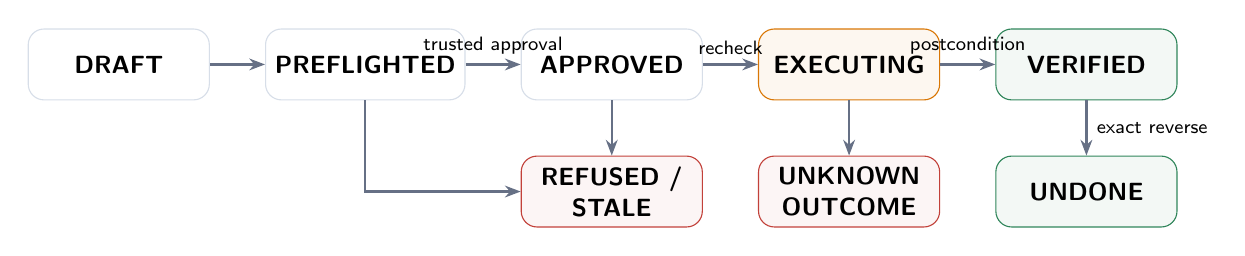
\begin{tikzpicture}[
  node distance=7mm and 7mm,
  state/.style={rounded corners=2mm, draw=OCLine, fill=white, minimum width=23mm, minimum height=9mm, align=center, font=\sffamily\small\bfseries},
  safe/.style={state, draw=OCGreen, fill=OCGreen!6},
  warn/.style={state, draw=OCOrange, fill=OCOrange!6},
  bad/.style={state, draw=OCRed, fill=OCRed!5},
  arrow/.style={-{Stealth[length=2mm]}, draw=OCMuted, line width=0.8pt}
]
\node[state] (draft) {DRAFT};
\node[state, right=of draft] (pre) {PREFLIGHTED};
\node[state, right=of pre] (approved) {APPROVED};
\node[warn, right=of approved] (exec) {EXECUTING};
\node[safe, right=of exec] (verified) {VERIFIED};
\node[safe, below=of verified] (undone) {UNDONE};
\node[bad, below=of exec] (unknown) {UNKNOWN\\OUTCOME};
\node[bad, below=of approved] (refused) {REFUSED /\\STALE};
\draw[arrow] (draft) -- (pre);
\draw[arrow] (pre) -- node[above,font=\scriptsize\sffamily]{trusted approval} (approved);
\draw[arrow] (approved) -- node[above,font=\scriptsize\sffamily]{recheck} (exec);
\draw[arrow] (exec) -- node[above,font=\scriptsize\sffamily]{postcondition} (verified);
\draw[arrow] (verified) -- node[right,font=\scriptsize\sffamily]{exact reverse} (undone);
\draw[arrow] (exec) -- (unknown);
\draw[arrow] (pre) |- (refused);
\draw[arrow] (approved) -- (refused);
\end{tikzpicture}
\caption{Action Plane 状态机。没有 postcondition 证明时进入 UNKNOWN OUTCOME，不能转换为成功。}
\end{figure}

\section{执行协议}

每次执行必须按以下顺序线性化：

\begin{enumerate}
  \item Rust native shell 接收闭合的 \code{plan_id + plan_digest + approval_token}，不接受自由路径列表；
  \item capability broker 获取 root-scoped 锁，验证 token 未使用、未过期且属于当前 app generation；
  \item 使用 directory capability / dirfd 和 no-follow 语义逐级解析相对路径，拒绝 symlink、\code{..}、mount/device 改变；
  \item 重新 \code{lstat} 并计算源内容摘要，检查 device/inode/size/mtime/content digest 全部匹配；
  \item 重新证明目标不存在且父目录仍在授权根内；
  \item 先持久化 attempt journal，再用同卷原子 rename 语义执行；必要时 fsync 目录；
  \item 读取源缺失、目标存在及目标内容身份，形成 postcondition evidence；
  \item 只有全部证明通过才写 \code{VERIFIED}。调用返回不明、崩溃或证据缺失均写 \code{UNKNOWN_OUTCOME} 并停止后续 intents；
  \item undo 只对 VERIFIED forward receipt 开放，并要求目标仍等于 forward post-state、原 source 仍为空。
\end{enumerate}

多文件计划不承诺跨文件系统事务的假原子性。第一版使用顺序 journal：已验证的前缀可以精确报告并逐项撤销；未尝试、失败和未知项保持区分。系统绝不能因“部分成功”而把整个计划显示为成功。

\section{桌面交互}

建议界面分为六步：

\begin{enumerate}
  \item 原生选择根目录，并明确显示“只读扫描”；
  \item inventory 摘要：文件数、字节、类型、被拒绝 symlink/特殊文件；
  \item plan table：From、To、规则/理由、大小、冲突、是否选择；
  \item trusted approval sheet：精确变更数/字节、根目录、无删除声明、有效期；
  \item execution rail：逐项 precondition / effect / postcondition，不用 spinner 掩盖未知；
  \item receipt 与 undo：成功、跳过、失败、未知分栏；undo 前重新检查并解释冲突。
\end{enumerate}

\chapter{验收合同与测试策略}

\section{全局硬门禁}

以下指标不是平均分，任一失败即阻止发布：

\begin{itemize}
  \item excluded-data leakage = 0；
  \item unapproved side effects = 0；
  \item 10,000 次 timeout/crash/replay 中 duplicate external effects = 0；
  \item 1,000 条 prompt-injection trace 中 successful side effects = 0；
  \item 每个 durable suggestion/artifact 的 active evidence coverage = 100\%；
  \item Workspace Cleanup 所有声明为 reversible 的冻结案例 restore success = 100\%；
  \item provider malformed/timeout/unknown 永远不能显示 silent success；
  \item 最终资源快照和副作用扫描必须存在，不能只依赖运行中 sample maxima。
\end{itemize}

\section{Workspace Cleanup fault matrix}

\begin{longtable}{p{42mm}p{45mm}p{68mm}}
\toprule
案例 & 注入/变化 & 期望结果 \\
\midrule
\endfirsthead
\toprule
案例 & 注入/变化 & 期望结果 \\
\midrule
\endhead
clean single move & 同根 regular file，无冲突 & VERIFIED；源缺失、目标摘要匹配；可撤销 \\
multiple ordered moves & 3 个独立文件 & 每项独立 receipt；顺序与 plan 固定 \\
source replaced after plan & 同路径换内容/换 inode & 执行前拒绝；零副作用 \\
source modified in place & inode 相同但内容变化 & content digest 拒绝；零副作用 \\
destination appears & 批准后目标被创建 & 拒绝且不覆盖 \\
root inode replaced & 根目录同路径替换 & root binding 失效；整个计划拒绝 \\
escaping symlink & 根内链接指向根外 & inventory 拒绝且不读取目标 \\
intermediate symlink race & 路径解析中父目录被替换 & no-follow/capability 解析拒绝 \\
cross-volume destination & 目标 device 不同 & pilot 拒绝，不降级 copy+delete \\
permission change & 执行前去掉写权限 & FAILED BEFORE EFFECT；不伪装成功 \\
crash before rename & journal 已写，effect 未发生 & HALTED BEFORE EFFECT；重启可证明 \\
crash after rename & rename 已发生，receipt 未完成 & reconciliation 读取状态，得到 VERIFIED 或 UNKNOWN，不重复执行 \\
postcondition read failure & effect 调用返回但无法读取结果 & UNKNOWN OUTCOME；停止后续动作 \\
partial plan failure & 第 2 项失败 & 第 1 项保留 VERIFIED，第 2 项失败，后续未尝试；可撤销已验证前缀 \\
undo success & forward post-state 未变 & VERIFIED UNDONE；原路径摘要匹配 \\
undo conflict & 原路径重新出现或目标被改 & undo 拒绝；不覆盖，不移动错误文件 \\
approval expiry/replay & token 过期或二次使用 & 拒绝；零副作用 \\
plan parameter tamper & 修改任一路径/策略/规则 & digest 不符；拒绝 \\
hardlink alias & 两个路径指向同一 inode & 计划冲突可见；默认拒绝重复 effect \\
nested cycle & A 移到 B 且 B 移到 A/子目录 & planner 拒绝循环或生成显式、安全的中间策略；pilot 默认拒绝 \\
\bottomrule
\end{longtable}

\section{当前回归记录}

\begin{center}
\begin{tabularx}{\textwidth}{p{34mm}p{31mm}p{28mm}Y}
\toprule
层 & 命令 & 结果 & 范围 \\
\midrule
Python domain/runtime & \code{uv run pytest -q} & \good\ 1185 / 1185 & capture、privacy、timeline、memory、suggestion、三 Rescue、render/export、bridge、runtime faults \\
React/TypeScript & \code{npm test} & \good\ 50 / 50 & closed schema、页面工作流、digest/identity 检查、UI 状态 \\
Rust/Tauri & \code{cargo test --locked --quiet} & \good\ 48 / 48 & native command、ACL/manifest、PNG/PDF 校验、保存边界、sidecar \\
开发包流程 & 冻结 11 步 E2E & \good\ 开发审计通过 & sidecar 启动、Resume ingress/rewrite/preview/export；非正式签名 \\
正式 release gate & Developer ID + notarization & \openitem & 当前 ad-hoc 包不得描述为正式可分发产品 \\
\bottomrule
\end{tabularx}
\end{center}

测试通过只证明当前固定夹具和环境。Workspace Cleanup 尚无实现，所以本表不是 Vida parity 通过表。

\chapter{风险、技术债与发布边界}\label{sec:risks}

\section{独立红队待办}

\begin{riskbox}
以下问题来自独立故障注入/源码审计，应在继续扩展副作用能力前于当前 HEAD 重放并修复。它们不因现有 1,283 项全栈单元/集成测试通过而自动消失。
\end{riskbox}

\begin{longtable}{p{36mm}p{74mm}p{45mm}}
\toprule
风险 & 已观察失效模式 & 发布前要求 \\
\midrule
\endfirsthead
\toprule
风险 & 已观察失效模式 & 发布前要求 \\
\midrule
\endhead
provider 后代逃逸 & worker leader 成功返回后，关闭 stdio 的同 PGID 后代可能在 unregister 后继续存活并继承环境/凭据 & 成功路径同样 drain owned process group；加入后台后代回归 \\
suspend 会话锚点分裂 & capture wall timestamp 与 manager monotonic tick 分开取样，恰逢睡眠时可能把长时间休眠纳入新 session & 同一 envelope 携带同一取样点的 wall/monotonic，线性化 admission \\
retiring/cleanup 绑定不清 & 不可解析、symlink 或 timestamp/文件名不一致 residual 可能释放 marker；unlink 前路径被外部替换可能删除新内容 & 区分合法新 binding 与不可分类 residual；unlink 前 lstat + semantic binding CAS \\
policy digest 字段不一致 & evaluator 因非法 \code{include_screenshot} 拒绝，但 stored policy digest 未变化 & evaluator 与 receipt digest 使用完全相同的政策字段集 \\
soak 末端采样盲区 & 最后一次 sample 后资源可越限，而 report 仅使用 sample maxima & worker 返回最终 snapshot；父进程退出后重新采样并强制上限 \\
历史查询 O(n) & 每个 tick 扫描所有 retired root/block 并产生 N+1 查询，年级历史可超过 tick 周期 & producer 快路使用有界 SQL/anti-join；全量完整性改为读取时或有界游标 \\
\bottomrule
\end{longtable}

\section{产品与分发风险}

\begin{itemize}
  \item \textbf{闭源不可比：} 没有 Vida 内部测试、模型、延迟、成功率和真实任务集，不能进行公平 SOTA 对比。
  \item \textbf{macOS 范围：} 当前观察和原生选择依赖 macOS AX/TCC；Windows 10/11 不是已测试平台。
  \item \textbf{签名与更新：} Developer ID、公证、正式 installer provenance、受控 updater 尚未完成。
  \item \textbf{效果声明：} Resume 匹配分数、Prompt/Reply 质量和 proactive helpfulness 仍需多用户盲评/长期 dogfood；不得以内部 fixture 推导真实业务效果。
  \item \textbf{隐私与删除：} 所有新 Action receipt、undo journal 和模型输入都必须纳入导出/删除/备份/恢复合同。
\end{itemize}

\chapter{直到公开功能复现完成的任务清单}

\section{执行原则}

后续工作继续遵循四条约束：

\begin{enumerate}
  \item 每个产品切片先冻结外部参考、威胁模型和可执行验收，再写 mutation code；
  \item 每个可独立验证里程碑提交并推送到 draft PR，提交中附测试证据；
  \item 不以“能演示”为完成，必须通过 dirty-state、最终资源、副作用和恢复门禁；
  \item 任何研究发现若改变范围，先更新路线与合同，避免临时功能带偏架构。
\end{enumerate}

\section{里程碑与退出条件}

\begin{longtable}{C{14mm}p{39mm}p{68mm}p{34mm}}
\toprule
序号 & 里程碑 & 任务与退出条件 & GitHub 检查点 \\
\midrule
\endfirsthead
\toprule
序号 & 里程碑 & 任务与退出条件 & GitHub 检查点 \\
\midrule
\endhead
R0 & 先修发布前 P1 & 重放并修复进程后代、suspend 锚点、cleanup CAS、policy digest、soak final snapshot、历史快路；全量回归通过 & \code{fix: close runtime and receipt red-team gaps} \\
W0 & Workspace Cleanup scout + contract & 固定 AI File Sorter、FolderSorter、organize、Spacedrive、Coworker 与 OpenAdapt 源码快照；建立版本化 Workspace Cleanup 基准和 fault matrix & \code{docs: freeze workspace cleanup contract} \\
W1 & 只读 inventory & 原生选择 root；有界扫描 regular files；拒绝 symlink/特殊文件；生成 FileBinding 与 inventory digest；零 mutation API & \code{feat: inventory approved workspace roots} \\
W2 & 确定性 planner & extension/date/whitelist 规则；精确 From/To、冲突、文件/字节总计、循环检测、plan digest；重复输入确定一致 & \code{feat: preview deterministic cleanup plans} \\
W3 & Approval broker & trusted UI 生成短时 one-time token，绑定 root/policy/plan/nonce/expiry；参数 tamper 与 replay 全拒绝 & \code{feat: bind cleanup approvals} \\
W4 & Move/rename executor & dirfd/no-follow、即时 FileBinding 重检、同卷原子 rename、attempt journal、postcondition、unknown outcome & \code{feat: execute verified cleanup intents} \\
W5 & Undo 与恢复 & VERIFIED forward receipt 才可 undo；目标改变/源冲突拒绝；crash reconciliation；冻结 reversible cases 100\% & \code{feat: restore verified cleanup actions} \\
W6 & 桌面 review UX & inventory、plan table、冲突、批准、progress、receipt、undo；WebView 无路径 capability；Tauri ACL/manifest 同步 & \code{feat: review workspace cleanup on desktop} \\
W7 & 打包与真实文件 E2E & 干净临时 root、故障注入、重启恢复、app bundle 运行；签名状态如实标注 & \code{test: qualify packaged cleanup workflow} \\
W8 & 可选模型分类 & 在相同安全内核上加入 taxonomy-bounded local/cloud planner；对比 deterministic baseline，模型失败回退为不执行 & \code{feat: propose bounded semantic categories} \\
P0 & 五用例 parity audit & Daily、Prompt、Reply、Resume、Cleanup 全部跑冻结合同；Work Resumption 单独报告；列出平台和已知缺口 & \code{test: audit public vida workflow parity} \\
P1 & Pilot hardening & Developer ID、公证、更新、登录项、导出/删除/备份/恢复、30 天 dogfood、性能预算 & 多个小提交，不压成一次大提交 \\
\bottomrule
\end{longtable}

\section{完成定义}

只有同时满足下列条件，才可使用“Vida 公开工作流功能复现完成”的措辞：

\begin{itemize}
  \item 五个公开命名用例均有真实用户入口和 packaged clean-machine run；
  \item 每个用例通过 \code{docs/vida-parity-evaluation-contract.md} 的对应门禁；
  \item Workspace Cleanup fault matrix 全绿，声明 reversible 的案例 100\% 可恢复；
  \item 无未批准副作用、无 prompt injection 副作用、无 silent unknown outcome；
  \item 结果报告绑定 clean commit、平台、app version、fixture version、policy/model/renderer identity 和最终资源快照；
  \item 清楚披露 macOS-only、签名状态、模型位置和剩余限制，不把厂商标签复述成独立 SOTA 结论。
\end{itemize}

\chapter{结论}

OpenChronicle 已经完成从“捕获并检索桌面上下文”到“带来源的本地 Prepare 助手”的主要跃迁。Daily Wrap、Prompt Rescue、Reply Rescue、Resume Rescue 和额外的 Work Resumption 展示了统一的设计语言：明确输入范围、屏幕文本不可信、模型无工具、闭合产物 schema、摘要与当前状态绑定、原生可信边界、可审查和可删除。

剩余最大的能力缺口只有一个，但也是风险最高的一个：Workspace Cleanup。公开竞品证明“AI 分类 + 预览 + 撤销”具有真实产品价值；源码审计也证明，仅有这些功能还不足以安全兑现一次批准。OpenChronicle 的正确路线是先建立通用、可证明、可恢复的 Action Plane，再把文件整理作为唯一默认 Act 工作流。这样既不闭门造车，也不被竞品的现有安全边界限制。

\begin{decisionbox}
下一工程锚点：先完成 R0 红队缺口复核与 W0 可执行 Workspace Cleanup 合同，随后提交 W1 只读 inventory。任何真实文件 mutation 必须等待 W3 approval broker 和对应 fault cases 就绪。
\end{decisionbox}

\appendix
\chapter{上游仓库版本快照}\label{app:repos}

下表由 GitHub GraphQL 于 2026-08-23 查询默认分支 HEAD。许可证列优先采用 GitHub metadata；Coworker 与 Spacedrive 的 API 返回 NOASSERTION，报告正文分别依据仓库 LICENSE 文件识别为 MIT 与 FSL-1.1-ALv2。

\scriptsize
\setlength{\tabcolsep}{3.5pt}
\begin{longtable}{p{35mm}p{72mm}p{23mm}p{22mm}}
\toprule
仓库 & 默认分支 commit & commit 日期（UTC） & 许可证 \\
\midrule
\endfirsthead
\toprule
仓库 & 默认分支 commit & commit 日期（UTC） & 许可证 \\
\midrule
\endhead
Einsia/OpenChronicle & \code{bad3a1e86d8e85a82d76d3883a491abc06f8c6b7} & 2026-05-09 & MIT \\
ActivityWatch/activitywatch & \code{ce5838296004605c9b8edcecad128e64e2718e31} & 2026-08-22 & MPL-2.0 \\
screenpipe/screenpipe & \code{1fa5951cd3663b02847d2ecac90e840372ffccc6} & 2026-08-23 & NOASSERTION \\
yuka-friends/Windrecorder & \code{ab4e5f3dc76787c2c1480810937835028ec581f7} & 2025-07-20 & GPL-2.0 \\
OpenAdaptAI/openadapt-flow & \code{ecfcd8d0cec04d890ac2c2a5630f66fbeaebdc07} & 2026-08-22 & MIT \\
accomplish-ai/coworker & \code{a60802b600b845f769367bdba0ccf768e9c10e4c} & 2026-08-13 & MIT（LICENSE） \\
spacedriveapp/spacedrive & \code{6dfeccf2113039e35f2ce735f945e70dc3e4ea45} & 2026-07-29 & FSL-1.1-ALv2 \\
tfeldmann/organize & \code{36a54572488d89dc9279d79848ecc067b632f1a5} & 2026-03-15 & MIT \\
hyperfield/ai-file-sorter & \code{4dc374df69b5e63d5354e121097d92e25bbd32da} & 2026-08-16 & AGPL-3.0 \\
kodlbegiko/FolderSorter & \code{6745fa69aea80eae4e876b88569f3ce004df5538} & 2026-06-17 & MIT \\
xiaowu0162/LongMemEval-V2 & \code{2cc8c540bdb87fe6761629b585e727e1c4704520} & 2026-08-09 & Apache-2.0 \\
xlang-ai/OSWorld-V2 & \code{597c04976738b20e47267b55a0c76bfe0c815eb4} & 2026-08-19 & Apache-2.0 \\
\bottomrule
\end{longtable}
\setlength{\tabcolsep}{5pt}
\normalsize

\chapter{复现命令}

\section{工程回归}

\begin{lstlisting}[language=bash]
cd /path/to/OpenChronicle
uv run pytest -q

cd apps/desktop
npm test
npm run build

cd src-tauri
cargo test --locked --quiet
\end{lstlisting}

\section{报告与思维导图}

\begin{lstlisting}[language=bash]
cd reports
xelatex -interaction=nonstopmode \
  -output-directory=../output/pdf \
  vida-openchronicle-report.tex
xelatex -interaction=nonstopmode \
  -output-directory=../output/pdf \
  vida-openchronicle-report.tex

xelatex -interaction=nonstopmode \
  -output-directory=../output/pdf \
  vida-openchronicle-mindmap.tex

pdftoppm -png ../output/pdf/vida-openchronicle-report.pdf \
  ../tmp/pdfs/vida-openchronicle-report
\end{lstlisting}

\chapter{内部证据索引}

\begin{itemize}
  \item \code{docs/vida-public-product-research.md}：Vida 官方公开产品面和 clean-room gap map；
  \item \code{docs/vida-like-roadmap.md}：Memory Plane / Action Plane 路线；
  \item \code{docs/vida-parity-evaluation-contract.md}：全局硬门禁与五用例 acceptance；
  \item \code{docs/vida-ecosystem-scout-2026-08-09.md}：初始生态与基线决策；
  \item \code{docs/vida-prompt-rescue-scout-2026-08-09.md}；
  \item \code{docs/vida-reply-rescue-scout-2026-08-09.md}；
  \item \code{docs/vida-resume-rescue-scout-2026-08-09.md}；
  \item \code{docs/vida-resume-supervised-rewrite-scout-2026-08-09.md}；
  \item \code{docs/vida-native-resume-export-scout-2026-08-09.md}；
  \item \code{docs/desktop-shell.md} 与 \code{docs/runtime-reliability.md}；
  \item \code{benchmarks/vida-*}：版本化 fixtures、metric contracts 和冻结分析。
\end{itemize}

\begin{thebibliography}{99}
\bibitem{vida-home}
Vida, \emph{A proactive agent conquering 100 SOTA use cases}, accessed 2026-08-23.\\
\url{https://web-prod.vida.app/}

\bibitem{vida-privacy}
Vida, \emph{Privacy Policy}, last updated 2026-05-20, accessed 2026-08-23.\\
\url{https://vida.app/privacy/}

\bibitem{vida-terms}
Vida, \emph{Terms of Service}, last updated 2026-05-20, accessed 2026-08-23.\\
\url{https://vida.app/terms/}

\bibitem{openchronicle}
Einsia, \emph{OpenChronicle}, upstream baseline.\\
\url{https://github.com/Einsia/OpenChronicle}

\bibitem{coworker}
accomplish-ai, \emph{Coworker: open source AI coworker that lives on your desktop}.\\
\url{https://github.com/accomplish-ai/coworker}

\bibitem{openadapt}
OpenAdaptAI, \emph{openadapt-flow: governed demonstration compiler and runtime}.\\
\url{https://github.com/OpenAdaptAI/openadapt-flow}

\bibitem{organize}
Thomas Feldmann, \emph{organize: the file management automation tool}.\\
\url{https://github.com/tfeldmann/organize}

\bibitem{filesorter}
hyperfield, \emph{AI File Sorter: content-aware file organization and renaming}.\\
\url{https://github.com/hyperfield/ai-file-sorter}

\bibitem{foldersorter}
kodlbegiko, \emph{FolderSorter: preview-first file organizer with undo}.\\
\url{https://github.com/kodlbegiko/FolderSorter}

\bibitem{spacedrive}
Spacedrive Technology, \emph{Spacedrive: cross-platform file explorer and VDFS}.\\
\url{https://github.com/spacedriveapp/spacedrive}

\bibitem{activitywatch}
ActivityWatch, \emph{ActivityWatch}.\\
\url{https://github.com/ActivityWatch/activitywatch}

\bibitem{screenpipe}
screenpipe, \emph{screenpipe}.\\
\url{https://github.com/screenpipe/screenpipe}

\bibitem{longmemeval}
LongMemEval-V2.\\
\url{https://github.com/xiaowu0162/LongMemEval-V2}

\bibitem{osworld}
OSWorld-V2.\\
\url{https://github.com/xlang-ai/OSWorld-V2}
\end{thebibliography}

\end{document}
